\begin{figure*}[t]
    \centering
    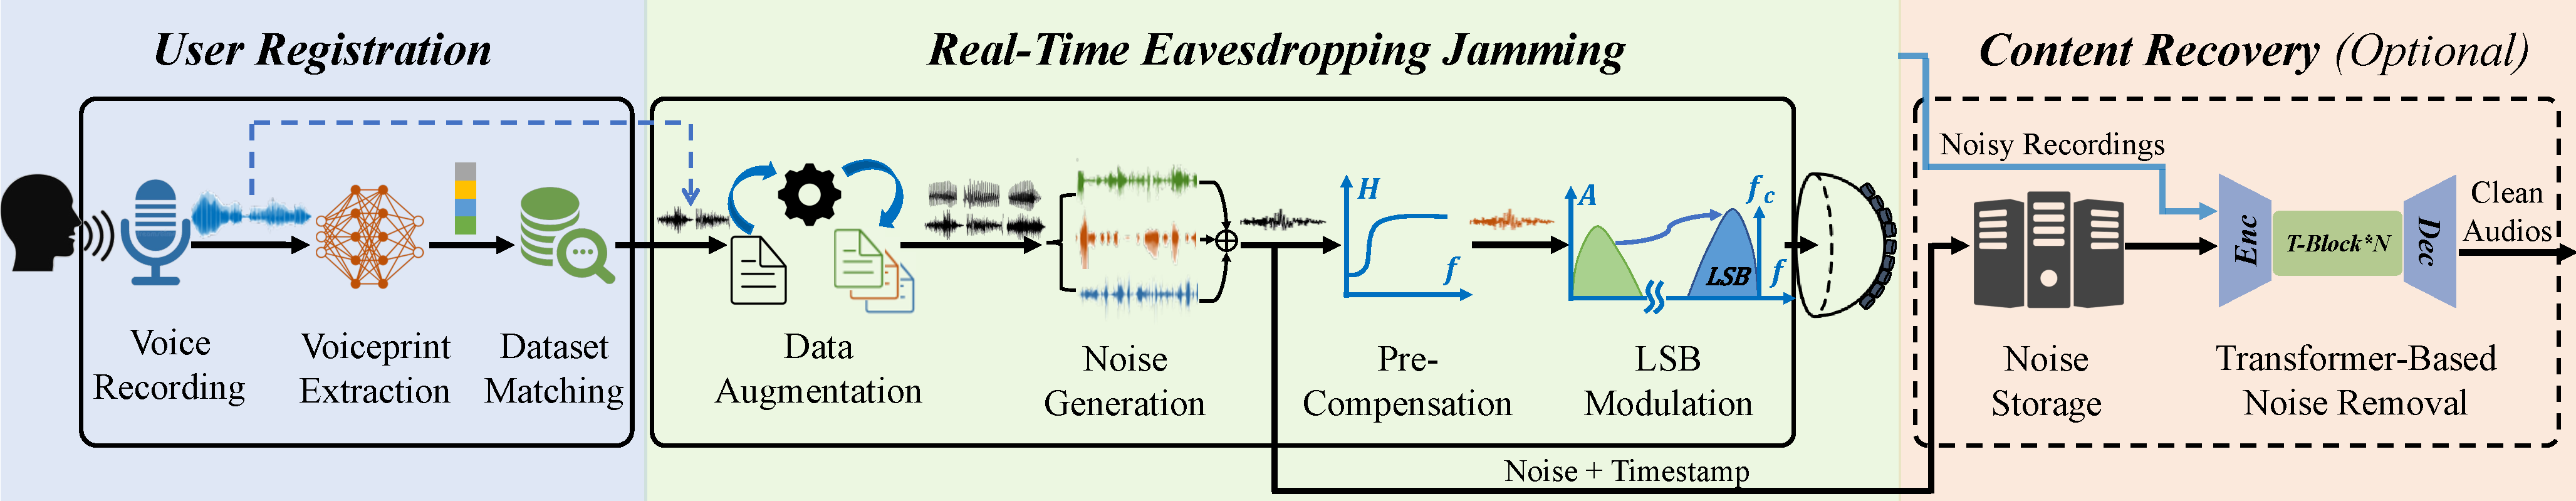
\includegraphics[width=\linewidth]{images/system_overview.pdf}
    \caption{Workflow of InfoMasker.}
    \label{fig:system_design}
    \vspace{-7mm}
\end{figure*}


\section{System Design}
\label{sec:system_design}

\subsection{System Workflow}

The workflow of InfoMasker is shown in Figure~\ref{fig:system_design}, involving three phases: \textit{User Registration}, \textit{Real-Time Eavesdropping Jamming}, and \textit{Content Recovery}. In the first, InfoMasker collects speech materials from user(s) and extracts their voiceprints. Depending on the amount of materials, it adopts different methods to generate adequate phoneme data.

The phoneme data is then used for noise generation in the second phase, in which InfoMasker continuously generates, compensates, modulates, and transmits the jamming noise to jam microphones in the environment.

If recording privilege is required, the noise will be stored with timestamps locally and fed into a denosing network together with noisy recordings to get clean audios.

\subsection{User Registration}
\label{subsec:user_registration}

As stated in Section \ref{sec:noise_design}, the phoneme-based noise is generated according to the user's speech data. However, collecting a large number of speech samples of the user is time-consuming thus sometimes not practical. Our solution is to pick speech data similar to the user's voices from a dataset. The similarity between the voices and the dataset audios is represented by the cosine similarity of their voiceprints, which are extracted with the method proposed in~\cite{GE2E}. Denote two voiceprints as $\bm{e_1}$ and $\bm{e_2}$, the cosine similarity of them can be represented as $1-d(\bm{e_1}, \bm{e_2})$, where $d(\bm{e_1}, \bm{e_2}) = \frac{\bm{e_1}\cdot \bm{e_2}}{||\bm{e_1}||||\bm{e_2}||}$.

To evaluate the effectiveness of this solution, we test three types of noise generated from audios showing different similarities to the user's voice: the user's voice, the audio with the highest similarity in a dataset, and the randomly chosen audios from a dataset. We also use WGN as a baseline. The dataset we used here is the train-clean-360 subset from LibriSpeech~\cite{LibriSpeech}. As shown in Figure~\ref{fig:jamming_with_other_data}, the jamming performance of the noises decreases as the voice similarity drops, and there is an about 10\% gap in Word Error Rate (WER) between the best and the worst case~\footnote[1]{In this paper we use Tencent ASR \cite{tencent_asr} for speech recognition if there is no special description}. Based on these results, we consider two types of registration scenarios according to the number of users.

\textbf{Single-User Registration. }
In this scenario, our priority is protecting a specific user's voice privacy. Meanwhile, the others' voices are also protected, merely with a 10\% drop in effectiveness as shown in Figure~\ref{fig:jamming_with_other_data}

There are two registration ways depending on the user's time availability. Given ample time, the user can record adequate speech data using Harvard Sentences dataset~\cite{harvard_sentences}, which contains phonetically balanced sentences. These recordings can provide sufficient and balanced phoneme data for noise generation. In contrast, when time is limited, the user can choose to record a few sentences for voiceprint extraction. Then the data with the most similar voiceprint in the dataset will be chosen for noise generation. 

To get the appropriate voice length for this time-restricted scenario, we conduct experiments to assess the impact of the voice length on the voiceprint similarity between the chosen data and the target people's voice (i.e., $d(\bm{e_{chosen}}, \bm{e_t})$). The results are shown in Figure~\ref{fig:test_registration_length} and the Ideal represents unrestricted voice length (utilizing all available data). We find that when voice length $<$ 5 seconds, the distance first drops rapidly as the length increases, and then drops much slower. The change in distance is neglectable when the length $>$ 5 seconds, indicating a 5-second speech is suitable for registration.

\begin{figure}[t]
    \centering
    \begin{minipage}[t]{0.49\linewidth}
        \centering
        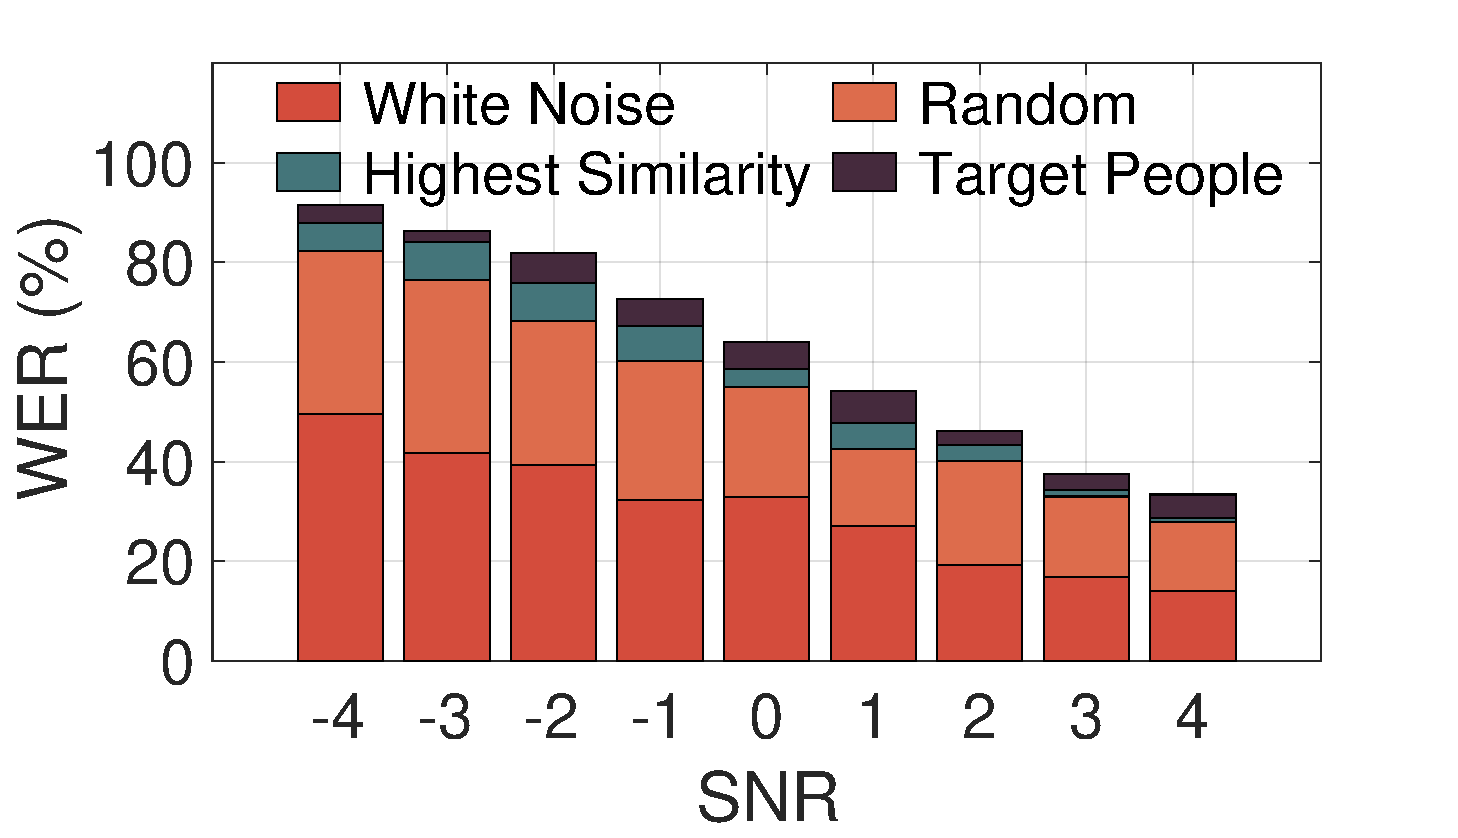
\includegraphics[width=\linewidth]{images/contrast_data.pdf}
        \caption{Effectiveness of different types of noise.}
        \label{fig:jamming_with_other_data}
    \end{minipage}
    \begin{minipage}[t]{0.49\linewidth}
        \centering
        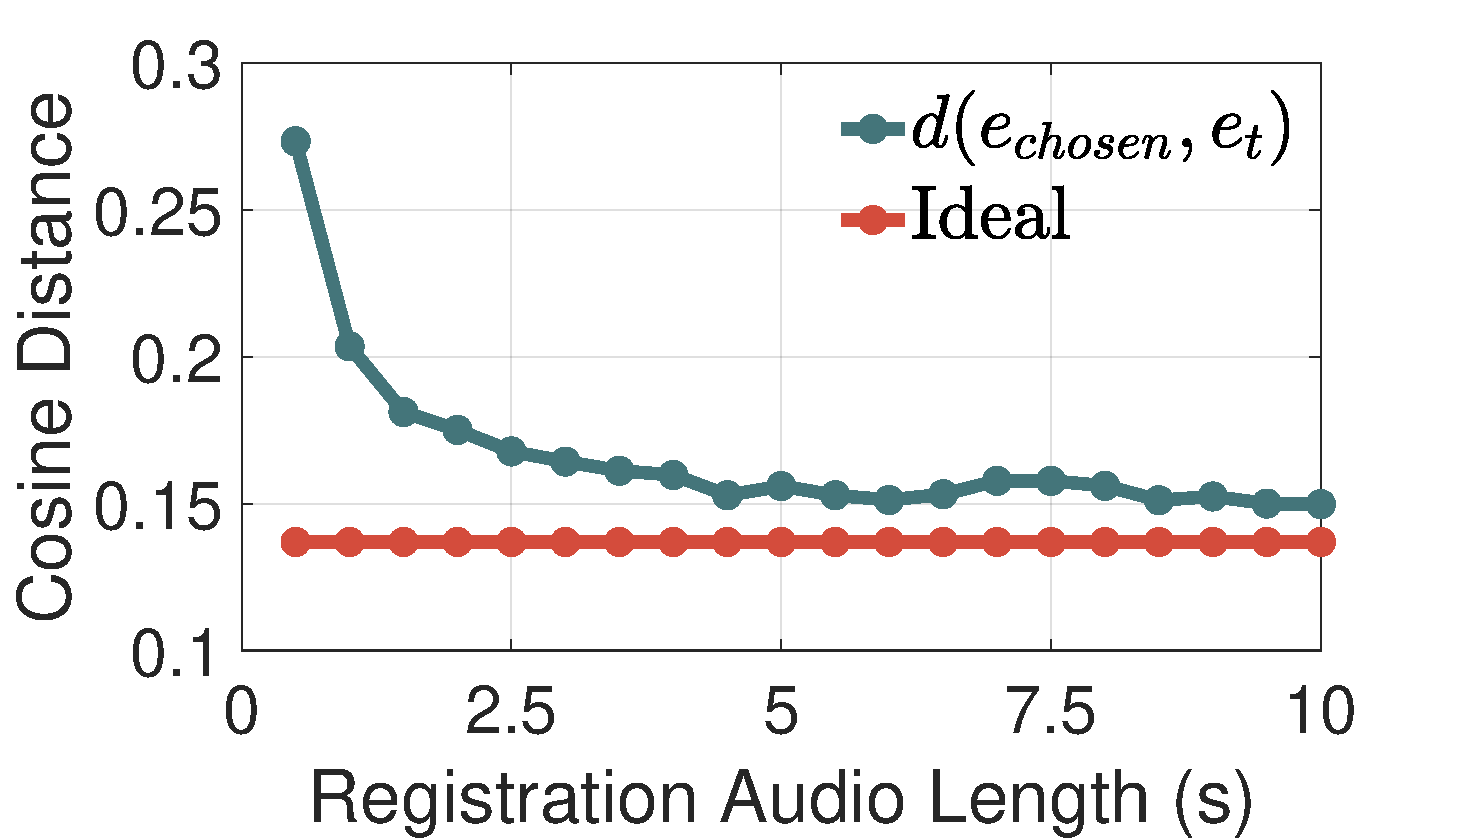
\includegraphics[width=\linewidth]{images/test_registration_length.pdf}
        \caption{Comparison of different registration speech length}
        \label{fig:test_registration_length}
    \end{minipage}
    \vspace{-5mm}
\end{figure}

\textbf{Multi-User Registration. }
In this scenario, we protect the voice privacy of all the people present in the environment. Similar to the time-restricted scenario for single user, the users need to record speech data with Harvard dataset for voiceprint extraction. As each user's voiceprint is different, here we use the average of each user's voiceprint as the representative feature for this group of people, then finds the best-matching data in the dataset for noise generation.

Please note that InfoMasker is totally offline during the usage, so the registration will not cause privacy leakage.

\subsection{Real-Time Eavesdropping Jamming}
After the registration, when InfoMasker is turned on to protect users' voice privacy, it will continuously augment the phoneme data, generate jamming noise based on these augmented data, and then emit the noise to the air to jam possible eavesdropping devices.

\textbf{Data Augmentation. }
With the data generated from the registration phase, we are now able to generate phoneme-based noise. However, since the amount of phoneme data is limited by the dataset, the probability of occurring recurring fragments in the noise will increase as more noise is generated, especially when the dataset is small. When an attacker locates these fragments, it is very possible for him to recover part of the semantic information from the recordings with the help of language models, similar to the key reused scenario in running key cipher. To prevent this, a data augmentation process that fine-tunes the phoneme data is applied to increase the total amount of data. To retain a high similarity between the augmented data and the original voices, the fine-tune should be restricted to a people's inner differences. Here we adopt the following properties used in emotion recognition~\cite{speech_emotion_detection}: speech rate, F0 mean, F0 contour, and energy, which have inherent inner differences because of people's different emotions, as shown in Table~\ref{tab:phonetical_properties}. In addition, we randomly reverse each single phoneme data, which has little effect on the data's phonetical properties but disrupts its semantic information.

\begin{figure}[t]
    \centering
    \includegraphics*[width=\linewidth]{images/data_augmentation.pdf}    
    \caption{Impact of data augmentation on the audio's phonetical features. The boxes illustrate the distribution of $d(\bm{\hat{e}}, \bm{e_t})$ where $\bm{e_t}$ is the target people's voiceprint and $\bm{\hat{e}}$ is the voiceprint of different types of audio.}
    \label{fig:data_augmentation}
    \vspace{-7mm}
\end{figure}

\begin{table}[H]
    \vspace{-3mm}
    \caption{Phonetical properties for data augmentation}
    \centering
    \resizebox{\columnwidth}{!}{
        \begin{tabular}{cccc}
        \toprule
        \multirow{2}{*}{\begin{tabular}[c]{@{}c@{}}Phonetical\\ Properties\end{tabular}} & \multirow{2}{*}{\begin{tabular}[c]{@{}c@{}}Modification \\ Range\end{tabular}} & \multicolumn{2}{c}{Emotional Impact}   \\ \cline{3-4}& & $\uparrow$ & $\downarrow$ \\ 
        \midrule
        Speech Rate     & 0.3-1.8 & Fear or Disgust        &  Sadness   \\
        F0 Mean      & 0.9-1.1 &  Anger or Happiness    & Disgust or Sadness  \\
        F0 Contour        & 0.7-1.3 & Anger or Happiness & Sadness \\
        % Speech Midpoint &    -    &    Anger or Happiness  &   Sadness    \\
        Energy          & 0.5-2.0 & -    & -     \\ 
        Sequential Order    &      -  & -    & -     \\  
        \bottomrule

        \end{tabular}
    }
    \label{tab:phonetical_properties}
    \vspace{-3mm}
\end{table}

\textit{Speech rate:} We change the original speech rate with a factor $\alpha$ using FFmpeg~\cite{ffmpeg} and $\alpha$ is uniformly sampled from $[0.3,1.8]$, which is obtained experimentally to guarantee an acceptable impact on phonetical properties. Please note that the change of speech rate here is independent of the acceleration of $S_1$ in the noise design, which aims to increase the number of vowels per unit time of our noise.

\textit{F0 mean:} Similar as before, we vary the F0 mean by a multiplicative factor $\alpha$ which is uniformly sampled from $[0.9,1.1]$. This range is also determined experimentally to limit the impact on phonetical properties.

\textit{F0 contour:} It shows the audio's pitch along with time. We exaggerate or flatten the F0 contour with $F0^{'} = \alpha(F0 - \overline{F0}) + \overline{F0}$ using World vocoder~\cite{world_vocoder}. The factor $\alpha$ is uniformly sampled from $[0.7, 1.3]$.

\textit{Energy:} We modify the average amplitude of the data with a factor randomly sampled from $[0.5, 2]$.

\textit{Sequential order:} For human speech data, the reverse in the time domain has little effect on phonetical properties but will disrupt the semantic information. In this paper, we randomly reverse each phoneme data in the time domain.

To visualize the impact of data augmentation, we extract voiceprints from each audio and calculate the cosine distance between them and the average voiceprint of the target people.
We compare four types of data: the data from the same people, from the people who have the closest voiceprint to the target people among the dataset (LibriSpeech train-clean-100~\cite{LibriSpeech}), the data processed by all five augmentation methods, and processed by every single method. Results in Figure~\ref{fig:data_augmentation} show that augmenting the data with a single method has limited impacts on its phonetical features. Even when augmented by all the five methods, the data is more similar to the original data than that of the closest people in the dataset. 

\textbf{Noise Generation.} With the augmented phoneme data, we now can generate noise with the method stated in Section~\ref{subsec:noise_design}. It should be noted that different from the origin method, the phoneme data used in this process could be either recorded from the target people, or matched from a pre-prepared dataset as stated in Section~\ref{subsec:user_registration}.

\textbf{Pre-Compensation.} Before we transmit the generated noise with ultrasound transmitters, it is necessary to compensate the noise signal due to the non-flat frequency response (FR) of transmitters. Figure~\ref{fig:transmitter_fr.pdf} illustrates a typical FR of a ultrasound transmitter~\cite{jinci} with a central frequency of 40 kHz, which exhibits a peak at about 40 kHz and rapidly attenuates as the frequency moves away. When transmitting noises with a carrier of 40 kHz (amplitude modulation), the low-frequency part will be promoted while the high-frequency part will be suppressed, as shown in Figure~\ref{fig:w_o_pre_compensation}, which could cause distortion of the noise thus decreasing the jamming effectiveness.

To address this, we analyze the FR of the recorder: $H_2(f)$, and the equivalent FR between the transmitter and the recorder: $H_1(f)$. The FR of the transmitter could be roughly estimated as $ H_1(f) * \frac{1}{H_2(f)}$. Then an inverse filter $h_1^{-1}(t) \ast h_2(t)$ \footnote[1]{$h(t) \xleftrightarrow {\mathcal{F}} H(f)$ means Fourier transform and $\ast$ means convolution.} is applied on the noise signal before modulation to compensate the unwanted distortion. We analyze $H_1(f)$ and $H_2(f)$ using multiple recorders and then adopt the average. Figure \ref{fig:w_o_pre_compensation} shows that the compensation works evidently. Please note that only the frequency blow 4kHz is considered for compensation as the majority of energy in human voice falls in this range. The drop below 1kHz in the ideal spectrum is caused by the recorders' imperfection.

\begin{figure}[t]
    \centering
    \begin{minipage}[t]{0.48\linewidth}
        \centering
        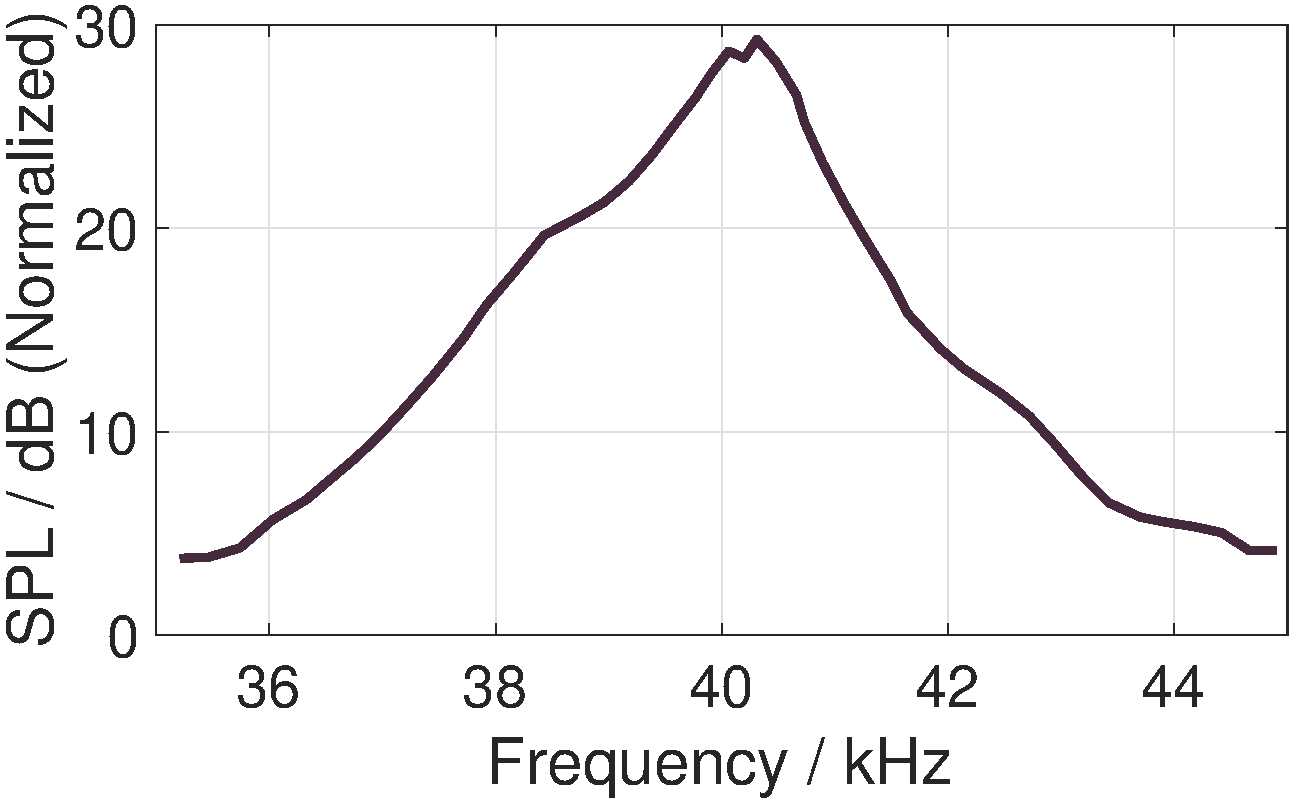
\includegraphics[width=\linewidth]{images/transmitter_fr.pdf}
        \caption{Frequency response of the transmitter.}
        \label{fig:transmitter_fr.pdf}
    \end{minipage}
    \begin{minipage}[t]{0.48\linewidth}
        \centering
        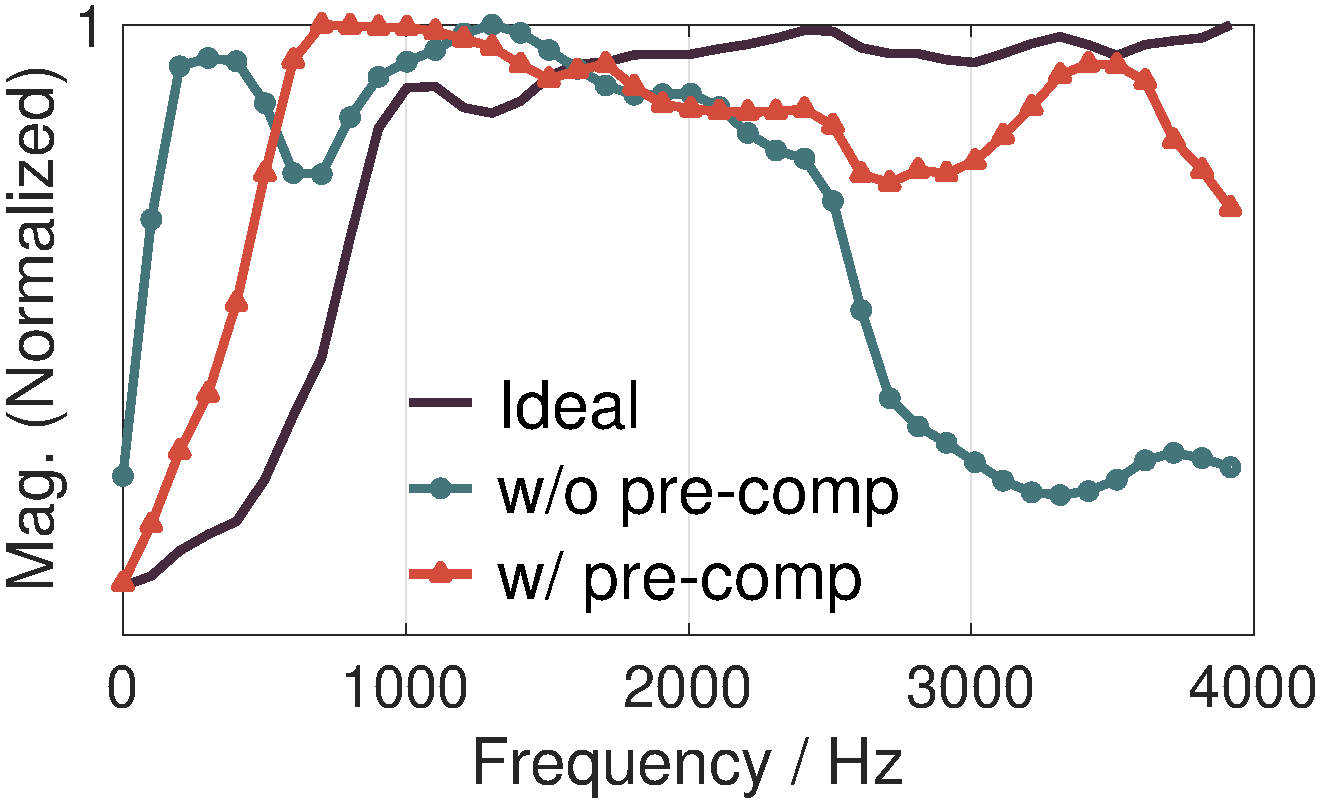
\includegraphics[width=\linewidth]{images/compensation.pdf}
        \caption{Spectrum of recorded sweep signals.}
        \label{fig:w_o_pre_compensation}
    \end{minipage}
    \vspace{-5mm}
\end{figure}

\textbf{Low-Sideband Noise Modulation.} 
With the compensated jamming noise, we now proceed to modulate it onto a carrier and transmit it via ultrasound transmitters to jamming microphones stealthily. However, the two widely used modulation methods, double sideband amplitude modulation (DSB-AM) \cite{10.1145/3133956.3134052,patronus} and frequency modulation (FM) \cite{backdoor}, are not suitable here. The wide frequency range of our noise results in a large bandwidth of the modulated signal if DSB-AM is applied, which increases the audibility of the noise because of the self-demodulation in the transmitter~\cite{backdoor, 211283}. As for FM, our phoneme-based noise cannot be recovered by self-demodulation at the receiver end.

In this paper, we use single-sideband modulation (SSB-AM) to reduce the noise audibility. Take the lower-sideband amplitude modulation (LSB-AM) as an example, assume the carrier signal is $cos(2\pi f_c t)$ and the noise signal is $n(t)$, then the DSB-AM can be represented by $n_D(t) = \sqrt{2}n(t) cos(2\pi f_c t)$ and the LSB-AM can be represented by $n_L(t) = n(t) cos(2\pi f_c t) + \widehat{n}(t) sin(2\pi f_c t)$, where $\hat{n}(t)$ is the Hilbert transform of $n(t)$ and $f_c$ is the carrier frequency. The coefficient $\sqrt{2}$ in the former is to ensure the energy of the two modulated signals are the same.
 
Similar to microphones, the nonlinearity in the ultrasonic transmitter also generates high order components. Because energy decays significantly as the order goes up, we only consider the quadratic term here. With DSB-AM and LSB-AM modulation, the quadratic terms of the modulated signal can be represented by Equations \ref{equ:DSB_qua} and \ref{equ:LSB_qua}. As shown in these two equations, the human audible low-frequency components for DSB-AM is $n^2(t)$, while for LSB-AM it is $\frac{1}{2}(n^2(t) + \widehat{n}^2(t))$. Because the Hilbert transform imparts a phase shift of $\pm \frac{\pi}{2}$ to each frequency component, the amplitude of each frequency component in the former is $\sqrt{2}$ times bigger than the latter. That is, the former has twice the energy of the latter which means SSB-AM can reduce the power of the audible sound generated at the transmitter to 0.5 times the original. 

\begin{equation}
    \begin{aligned}
     n^2_{D}(t) = &n^2(t)(1+cos(4\pi f_c t))\xRightarrow[Filter]{Lowpass} n^2(t)
    \end{aligned}
    \label{equ:DSB_qua}
\end{equation}
\begin{equation}
    \begin{aligned}
        n^2_{L}(t) \xRightarrow[Filter]{Lowpass}0.5(n^2(t) + \widehat{n}^2(t))
    \end{aligned}
    \label{equ:LSB_qua}
\end{equation}

Additionally, we choose lower-sideband instead of higher-sideband because of its lower attenuation in the air. The $f_c$ we used is 40 kHz, which has the maximum resonance response in most microphones~\cite{backdoor}.

We conduct an experiment with 3 males and 3 females aged from 22 to 31~\footnote[1]{All procedures performed in studies involving human in this paper are validated through an institutional review (IRB)} to test the impact of modulation methods on audibility.
We gradually increase the transmission power until volunteers perceive the noises. The normalized maximum transmission energy is shown in Table~\ref{tab:self_demodulation}.

\begin{figure}[t]
    \centering
    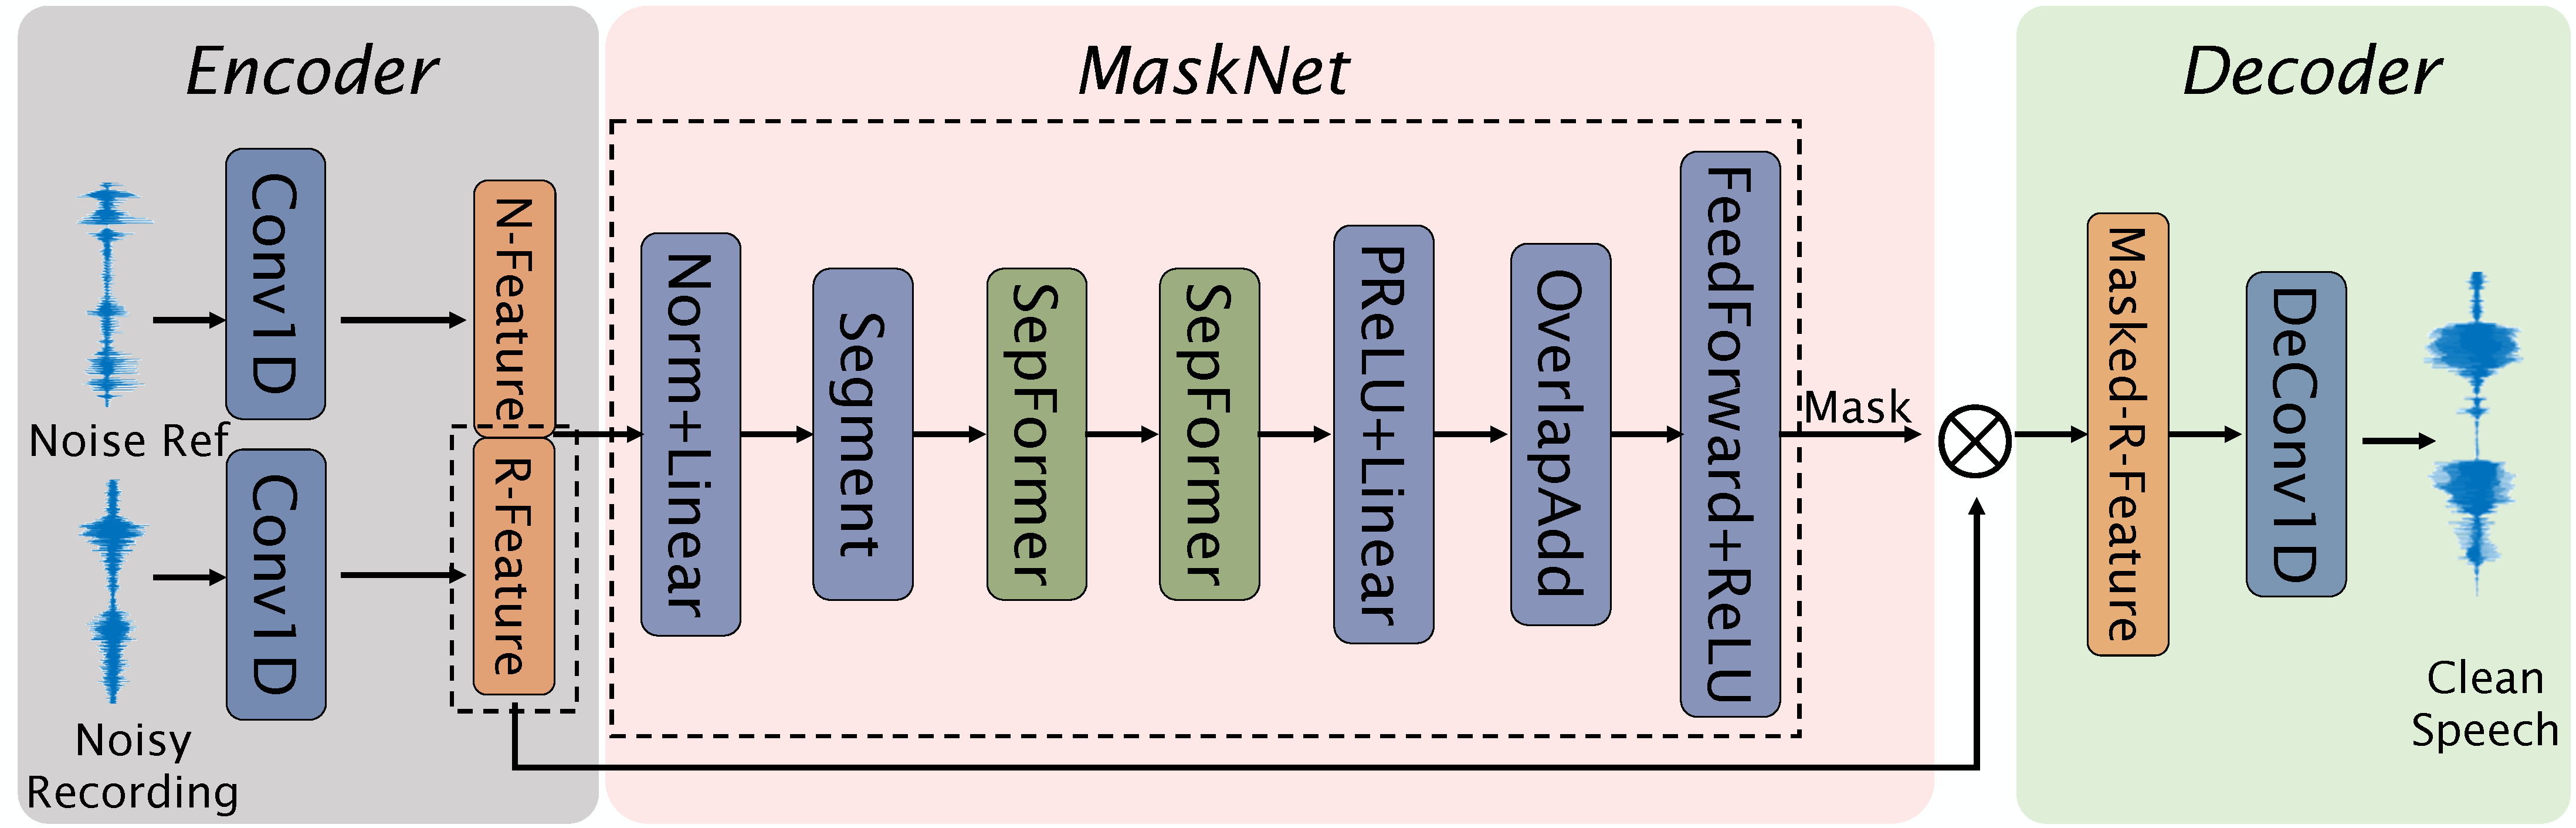
\includegraphics[width=\columnwidth]{images/network_architecture.pdf}
    \caption{Network Architecture}
    \label{fig:network_architecture}
\end{figure}

\begin{table}[t]
    \centering
    \resizebox{0.9\columnwidth}{!}{
    \begin{tabular}[\textwidth]{cccc}
        \toprule
        \multirow{2}{*}{Noise} & \multicolumn{3}{c}{Normalized Energy} \\ \cline{2-4} 
                               & DSB-AM      & LSB-AM     & USB-AM     \\ 
        \midrule
        White Noise            & 1.00        & 1.49       & 1.29       \\
        Phoneme-Based Noise    & 2.77        & \textbf{4.14}       & 3.61       \\ 
        \bottomrule
    \end{tabular}}
    
    \caption{Normalized max transmission energy.}
    \label{tab:self_demodulation}
    \vspace{-5mm}
\end{table}

\subsection{Content Recovery}
In certain situations, users may need to record the ongoing conversation while ensuring protection against adversaries. However, all microphones within the environment would be affected by InfoMasker, resulting in noisy recordings for both adversaries and users. 

To address this problem, we plan to eliminate the jamming noise from noisy recordings with the help of deep-learning model. Specifically, assume the ongoing speech is $s(t)$ and the transmitted jamming noise is $n(t)$, the noisy recording could be represented by:
$$
r(t) = s(t) + \alpha \cdot h_{1}(t) \ast n(t) + a(t)
$$
where $h_{1}(t)$ is the combination of channel impulse response (CIR) caused by over-the-air transmission and the residual distortion of the compensation process for the jamming noise. $a(t)$ represents the ambient noise. $\alpha$ is an unknown coefficient representing the amplification factor of the noise. 

Our target is to acquire $s(t)$. Our main idea is to remove noise components (i.e., $\alpha \cdot h_{1}(t)\ast n(t) + a(t)$) from noisy recordings $r(t)$. Because adversaries only have access to $r(t)$, it is hard for them to recover $s(t)$, while it is possible for the user with the help of the detail of the jamming noise signal $n(t)$. InfoMakser could store these noises along with timestamps while jamming recorders. This additional information makes it possible to recover $s(t)$.

\textbf{Network Architecture.} To achieve this target, we design a transformer-based denosing network based on~\cite{sepformer}. The network takes the noisy recording and the clean noise reference as inputs, generating clean audios as the output, as illustrated in Figure~\ref{fig:network_architecture}, which contains three parts: encoder, masknet, and decoder. The encoder employs two convolution layers to convert input audios to 2-D feature maps. Then the feature maps of the noisy recording and the noise reference are concatenated and fed into the masknet. The masknet contains two SepFormer blocks that can focus on both short- and long-term audio features, enabling it to find connections between these two feature maps and generate a mask to filter out noise components from the noisy recording's feature map. The decoder is symmetrical to the encoder. containing deconvolution layer and converting masked audio feature maps to clean audios.

We adopt the scale-invariant signal-to-noise ratio (SI-SNR)~\cite{si-snr} as the loss function, as shown in Equation~\ref{equ:sisnr}. Compared with the SNR metric, SI-SNR is more robust, scale-invariant, and can characterize the speech quality.

\begin{equation}
    \mathcal{L}_{\text{SI-SNR}}(s, \hat{s}) = -10 \text{log}_{10} \left( \frac{||\frac{\hat{s}^T s}{||s||^2}s||^2}{||\frac{\hat{s}^T s}{||s||^2}s - \hat{s}||^2} \right)
    \label{equ:sisnr}
\end{equation}

\textbf{Training Process.} There are two main challenges recovering the clean audio: \textbf{\textit{Time-domain misalignment}}: There are two reasons account for this. The first is that it takes different time for the voice and the jamming noise to arrive at the recorder. For example, the difference of 1 meter in transmission distance can make the error between two timestamps up to $1/340\approx0.0029$ seconds, about 139 sampling points (48 kHz). And the second is that the timestamps of audio recordings are often coarse.
% And the second reason is that although the digital domain jamming noise could be stored with timestamps, these timestamps are often coarse. 
For example, the recording timestamp in iOS 16.1 (iPhone 14) and Android 12 (Redmi K30Ultra with MIUI 14.0.1) is often accurate to second, which means the error could be up to 48000 sampling points under a 48 kHz sampling rate.
\textbf{\textit{Unknown channel impulse responses}}: The usage environment of InfoMasker could be various, which means the channel impulse responses of the target speech signal and the jamming noise are uncertain and could differ significantly from each other. So we can not preset $h_{1}(t)$ in the training process.

To cover the first challenge, we introduce a random shift in the noise reference in the training process, and the shift interval is [-fs, fs] where fs is the audio sample rate. The random shift will force the network to align the noisy recording and the reference automatically. While for the second, we leverage several public acoustic CIR datasets, including~\cite{AIR, RWCP, SPARG}, and randomly choose $h_{1}(t)$ from them for each training step. The abundant CIR data in the training process could help the neural network learn characteristics of reverberation and eliminate the effect of reverberation when generating the mask.
